\documentclass{article}
\usepackage{url}
\usepackage[T1]{fontenc}
\usepackage[french]{babel}
\usepackage{enumitem}
\usepackage{amssymb}
\usepackage{textcomp}
\usepackage[utf8]{inputenc}
\usepackage{graphicx}
\usepackage{geometry}
\usepackage[hang,small]{caption}
\geometry{hmargin=2.5cm,vmargin=2.5cm}
\frenchbsetup{StandardLists=true} % à inclure si on utilise \usepackage[french]{babel}

\title{TPE}
\date{2018}
\author{Gwendal Richomme, Julien Pommerol, Mathieu Burbaud}

\begin{document}

\section{Geology}

Cave's Geology

\subsection{Subsection}

Structuring a document is easy!

\subsubsection{Subsubsection}

More text.

\paragraph{Paragraph}

Some more text.

\subparagraph{Subparagraph}

Even more

\newpage

\section{Biology}

\subsection{Cave’s conditions}

We are gonna now approach the question of life in caves. For a long time in history, we have thunk that caves were almost empty, except rare specimens of fish, small amphibians or mammals such as bats. However, we now know that reality is pretty different. We have yet discovered about 50,000 species of cave animals. And we are still discovering new of them. For instance, in 2018, Chinese scientists discovered a cave beetle, whose has now the name of \emph{Xuedytes bellus}.
\smallbreak
To deal with cave’s species, we have first to talk about cave’s climatic conditions: when caves are long and deep enough, they are able to develop their own micro-climate. Dr Gheorghe Racoviță, a Romanian scientist has described three different micro-climates into the caves.

\begin{itemize}[label=$\square$]
  \item The \textbf{disturbance micro-climate}, or \textbf{entrance zone}, concerning the entrance of the cave, is characterized by numerous exchanges with the surface. For instance, the air fluctuation amplitude, with a temperate climate, is about 18.8°F (10°C), whereas it is usually of about 55.4°F (13°C). In this part of the cave, we can find green vegetation, because the luminosity rate is pretty high

  \item The \textbf{transitional micro-climate}, or \textbf{twilight zone}, concerns the part of the cave where the air fluctuation amplitude is less than 18.8°F (10°C) in temperate climate. Only a few resistants plants survive here.

  \item The \textbf{stability micro-climate}, called also \textbf{dark zone},  as its name indicates, is the deeper zone of the cave, where the air fluctuation is reduced to less than 1,8°F(1°C), and where there is no more light.

\end{itemize}
\begin{figure}[!ht]
  \centering
  \includegraphics{Images/Cave_zones}
  \caption{The zones of the cave \cite{CaveZones}}
  \label{Cave_zones}
\end{figure}

\newpage

We can’t define a precise average temperature of the caves. Indeed, this temperature depends of two factors. First, it depends of the cave’s location, and therefore of the atmosphere temperature. Then the temperature can vary with the depth of the cave. The heat of Earth plays actually a crucial role in cave’s climate. The average of these two factors determines the temperature of the cave. Usually, the caves are not located so deep. That’s why the temperature of the cave is often the same as the average temperature of the surface.
\smallbreak
However, cave humidity is really high, compared to the surface, because it is above 90 \%, against about 70 \% in the region Languedoc-Roussillon.
\bigbreak
Even if describing air circulation in caves seems difficult, because of the variations due to the external air circulation, scientists reached to find three types of air displacements, or circulation. To obtain models, they used tracer gases such as SF6 and CCl2F2 and determine their trajectory \footnote{Tracer gas: color and odorless gas, inert, non-toxic, that can’t displace air, and which is usually not present in the air and can,t be mistakable for other gases}. Here are the three different models of air-circulation that they obtained:
\begin{itemize}[label=$\square$]

  \item The \textbf{unidirectional (one-way) air circulation}. When a cave possesses only one entry, the warmer air, located deeper, rises up.  At the same time, the colder air flows in at the floor of the cave. This forms an air current. The deeper the cave is, the more powerful the air current is. This unidirectional air circulation can also cause the formation of “\textbf{cold traps}” . In temperate climate, during winter, the cooler air flows in the colder parts of the cave. Then, the rocks around become slowly colder. The rocks retain this coldness several 	months. Consequently, in summer, they are still cool when the water coming from the leaking ices outside flows into the cave. Finally, by being in contact with these cold rocks, water transforms into ice. That is why we can find huge ice formations in some caves, like in “The Mer de Glace” in France.

  \item The \textbf{bidirectional air circulation (two-ways)}. To have these kind of circulation, the cave must possess at least two entrances. Because of the difference of temperature between outside and inside the cave, air movements are created, particularly in Winter and Summer, when this difference is higher. Indeed, in Winter, the cold air comes into the cave by using the lower entry. Then, inside the cave, it warms up and rises up to go away at the upper entrance of the cave. In Summer, this process is inverted. \par
  Like in the case of the unidirectional air circulation, when the cave is located very high, the rocks of the lower part of the cave sustain the cold in Winter, and in Summer, when water flows, it turns into ice at this level. If these ice is perennial, that is to say if the ice is present in the cave all the year long, the cave is called a \textbf{dynamic ice cave}.

  \item The \textbf{multi-directional air circulation (numerous-ways)}. When caves possess many entrances, even little ones. Actually, the movements due to \textbf{chimney air flows} occurs. In winter, the warm air situated in caves leaves the cave. It is immediately replaced by colder air. In summer, this process occurs but is inverted, that is to say cold air leaves and warm air enters in the cave.

\end{itemize}

\begin{figure}[!ht]
  \centering
  \includegraphics[scale=1.5]{Images/Illustrations-of-mechanisms-for-cave-airflow-For-thermally-driven-flows-airflow}
  \caption{Aiflows in caves
    \\ a) and d) multi-directional air circulation
    \\ b) and c) unidirectional air circulation
    \\ e) and f) bidirectional air circulation \cite{CaveAirCirculation}}
    \label{Airflows}
\end{figure}

\clearpage

\subsection{Lifeforms in caves: their physiology and behaviours}

As we have seen, the life conditions in caves are really hard. At first sight, life seems impossible in such a environment, the dark zone, meaning the deepest and darkest part of the cave. However, life finds always a way to develop itself. That’s why we can find many types of lifeforms in caves. We can class them into four types:

\begin{itemize}[label=$\square$]

\item \textbf{Cavernicoles} are animals which live in dark environments, for instance caves. They are mainly arthropods, i.e. crustaceans, centipedes, millipedes, spiders, scorpions and insects.

\item \textbf{Troglophiles} (Greek for “who like caves”) are the animals that often live in dark environments, like caves, but are able to adapt themselves to live outside, in other middles with more light.

\item \textbf{Trogloxenes} (Greek for “foreign to caves) live only a part of their life cycle inside caves. They often go inside caves to sleep. These explore just the entry of the caves, where there is light. They are not particularly adapted to cave’s life, even if they can possess metabolisms that are also adapted for cave’s life (for instance echolocation). These animals are often the biggest in the cave. They include amphibians, small mammals like rats or bats. Humans, at the beginning of History were also trogloxenes.

\begin{figure}[!ht]
  \centering
  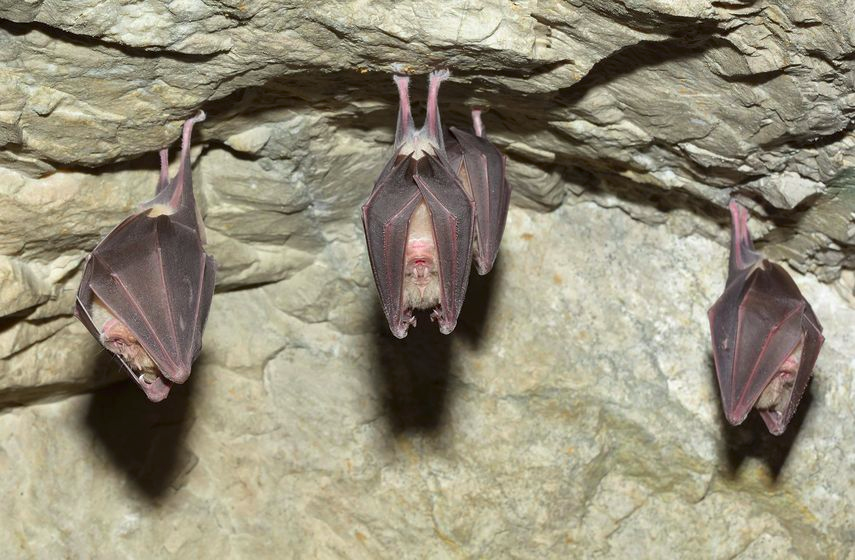
\includegraphics[scale=0.5]{Images/bats}
  \caption{Bats: troglophiles and trogloxenes \cite{BatsPresentation}}
\end{figure}

\item \textbf{Troglobites} (Greek for “cave dwellers”) have been living in the caves for a very long time. Therefore, they changed to adapt the hard conditions of life. These animals can not live outside cave’s environment. They are often small amphibians or insects and arachnids like cave spiders or cave crickets and pseudoscorpions. We can also find centipedes, and even fishes that are troglophiles, damned to live their entire life into caves.
\end{itemize}

\begin{figure}[ht]
    \begin{minipage}[c]{.46\linewidth}
        \centering
        \includegraphics[scale=0.6]{Images/Cave_beetle}
        \caption{Troglobite fish \cite{CaveBeetle}}
    \end{minipage}
    \hfill%
    \begin{minipage}[c]{.46\linewidth}
        \centering
        \includegraphics[scale=0.6]{Images/Cave_fish}
        \caption{Troglobite cave beetle \cite{CaveFish}}
    \end{minipage}
\end{figure}

Normally, insects or fish can not grow into caves. They will not indeed by their own go down into the caves. Now, how can they be all the same present in almost closed cave environment? The scientists have found some explanations. First, the animal could have migrated millions of year ago, during the ice ages. They had indeed to find heat to survive. Consequently they went into the caves, and adapted themselves. When the ice age ended, they could not rise up to the surface, and were trapped into caves. Secondly, it can happen during summer, that when ice sheets melted, small animals are brought with water and fall into caves.
\\
Cave’s organism act differently and adapt different physiology. These are due to the high lack of food in caves, compared to the surface, and the limited size of the caves. Here are the main physiology’s differences between surface and cave-dwelling species:

\begin{itemize}[label=$\square$]
  \item \textbf{Higher lifetime}. Organisms in caves often have a very long lifetime, compared to similar surface-dwelling creatures. For instance, a 20-30 centimeter long salamander, called cave olm can live until 80 years. Surface-dwelling salamander can live a maxima 30 years in their natural environment.\par
  Now, this high lifetime is due to many causes:
  \begin{enumerate}
    \item An higher resistance against starvation, caused by the lack of food supplies compared to the surface.
    \item A modified metabolic rate , that is to say energy used by organism per unity of time.
    \item An altered circadian cycle, i.e. the different metabolisms higher rate per day. Caves’ organisms are not disturbed by many factors like luminosity, temperature, or humidity, because they are located in places with no changes: cave’s darkest zone. (can also be an absence of circadian cycle).
      \begin{figure}[!ht]
        \centering
        \includegraphics[scale = 0.4]{Images/Circadian_Cycle}
        \caption{Man circadian cycle \cite{CircadianCycle}}
      \end{figure}
  \end{enumerate}
  \item \textbf{Lower fecondity}. Because of the lack of food, species like LABIDOGNATHA Liocranidae Brachyanillus, Liocranum and Agraecina, cave spides, do not spawn as many eggs as surface-dwelling species (less than 10 eggs). Moreover, these eggs are smaller (eggs’ side = 12.3mm for cave spiders against 16.8mm for surface spiders)
\end{itemize}

Besides, caves’ species behaviour are really different compared to other surface-dwelling species. Unfortunately, a few is known about cave’s organisms’ behaviours, because not a lot of observation were made. Many behaviours like reproduction, aggression,  aggregation seem to be the same as one’s of surface-dwelling species.
\par
For spiders (like  LABIDOGNATHA Liocranidae Brachyanillus, Liocranum and Agraecina), we can notice a change. Indeed, this creature do still produce webs. But in caves, this is more to act as a secured refuge for spiders. To chase, they do travel around the cave, searching preys.
\par
However, living in cave also reduce the adaptability of organisms to environments data (temperature, humidity, luminosity), because organisms are so well-adapted to their own cave’s conditions, that they can not support any changes.

\textbf{add Julien's work}

\clearpage

\subsection{Food Chain}

As all  the ecosystems, inside the cave, we find predators and preys. Here we are gonna explain you these Food Chain. \\
\par
At the bottom of the pyramid, we find mainly bacteria, often chemoautotrophic, heterotrophic and at the entry of the cave photothopic. We also find litter from the trogloxenes like bats’ guano and fungi. The chemoautotrophic bacteria produce their own organic matter by using chemical rections. Heterotropics bacteria, such as \emph{Synechococcus elongatus} and \emph{Anacystis montana}  and fungi use rather readymade organic food molecules. Some Fungi like \emph{Armellia mellea}, \emph{Xylaria hypoxylon} and \emph{Xylaria polymorpha} or \emph{Poriaillanti} are wood-parasites, whereas \emph{Paecilomyces} grows on dead insects, and both \emph{Beauveria} and \emph{Hirsutella} develop on living insects, that they killed after feeding of insect’s organic matter. \\
\par
Then we find mainly arthropods and lot of troglobites creatures, which eat the fungi and the organic matter delivered by bacteria. Here there are mainly, millipedes (ex: \emph{Polydesmus angustus} or \emph{Brachydesmus superus}) or small crustaceans (ex: \emph{Niphargus fontanus}). \\
\par
The last step of the food chain pyramid is the predator’s one. Here we find the biggest animals like salamandres (ex: \emph{Eurycea lucifuga}), spiders (ex: \emph{LABIDOGNATHA Liocranidae Brachyanillus}, \emph{Liocranum} and \emph{Agraecina}), pseudoscorpions (ex: \emph{Roncus lubricus}), mites (ex: \emph{Calyptostoma velutinus}), fishes (ex: \emph{Astyanax jordani}) and also tiny poisonous animals like centipedes (ex:\emph{ Lithobius microps}). In Alpen can we find the strange \emph{cave olm}, who is the biggest predator of the caves where it lives. \\
\par
The main part of the trogloxenes chase outside from the caves, like bats.

\begin{figure}[!ht]
  \centering
  \includegraphics[scale=0.6]{Images/Food_chain}
  \caption{Cave's food chain \cite{FoodChainPyramid}}
\end{figure}

\subsection{Metabolisms}

Lifeforms

\subsection{Human impact on the ecosystem}

Human impact on the ecosystem
\nocite{*}
\bibliographystyle{plain}
\bibliography{sitography}
\end{document}
